\documentclass[aspectratio=169]{beamer}
\usetheme{Madrid}
\usecolortheme{seahorse}
\usepackage{hyperref}
\usepackage{amsmath,amssymb}
\usepackage{tikz}
\usetikzlibrary{arrows.meta,positioning}

\title{A3 + The Slop Feedback Loop}
\author{Halley Young}


\setbeamertemplate{navigation symbols}{}
\setbeamertemplate{footline}[frame number]

\begin{document}

\begin{frame}
\titlepage
\end{frame}

\begin{frame}{1. Deliverable first}
\begin{itemize}
  \item \texttt{pip install a3-python} ships a static-first bug finding pipeline
  \item Stage 1: discover + prove/disprove + eliminate with auditable evidence
  \item Stage 2: send only unresolved residue to agentic triage
  \item Core design: deterministic elimination first, LLM judgment last
\end{itemize}
\end{frame}

\begin{frame}{2. One ridiculous origin story (from the blog)}
\begin{itemize}
  \item Started as a challenge: can AI generate verification theory that survives implementation?
  \item Early output: elegant quantitative semantics, weak execution contact
  \item Project inversion: ideas survive only if executable and regression-stable
  \item Blog thesis: ``fight AI slop with AI slop'' \(\rightarrow\) adversarial testing loop
\end{itemize}
\end{frame}

\begin{frame}{3. Episode I: distance-to-safety intuition}
\begin{itemize}
  \item Quantitative view: safety as distance \(d(\sigma,U)\), not only Boolean verdict
  \item Useful for prioritization and triage ordering
  \item Insufficient alone for production false-positive collapse
  \item Transition pressure: from ranking uncertainty to proving unreachability
\end{itemize}
\end{frame}

\begin{frame}{4. Episode II: prove unsafe is unreachable}
\begin{itemize}
  \item Reachable set \(R\), unsafe set \(U\), target claim: \(R \cap U = \varnothing\)
  \item Synthesize separator certificate \(B\) with inductive side conditions
  \item If obligations hold, candidate bug is provably infeasible (high-confidence FP elimination)
  \item If obligations fail, route to refinement or alternate proof family
\end{itemize}
\end{frame}

\begin{frame}{5. Barrier obligations (informal form)}
\begin{block}{Certificate constraints}
\[
\forall s\in S_0: B(s)\ge\epsilon,\quad
\forall s\to s': B(s)\ge0 \Rightarrow B(s')\ge0,\quad
\forall s\in U: B(s)\le-\epsilon
\]
\end{block}
\begin{itemize}
  \item Initialization, consecution, unsafe separation must all hold
  \item Solver outcomes interpreted conservatively: UNSAT prune, SAT keep, UNKNOWN keep
  \item Obligation failure provides a refinement signal, not silent drop
\end{itemize}
\end{frame}

\begin{frame}[shrink=2]{6. One certificate mapped to one Python bug}
\centering
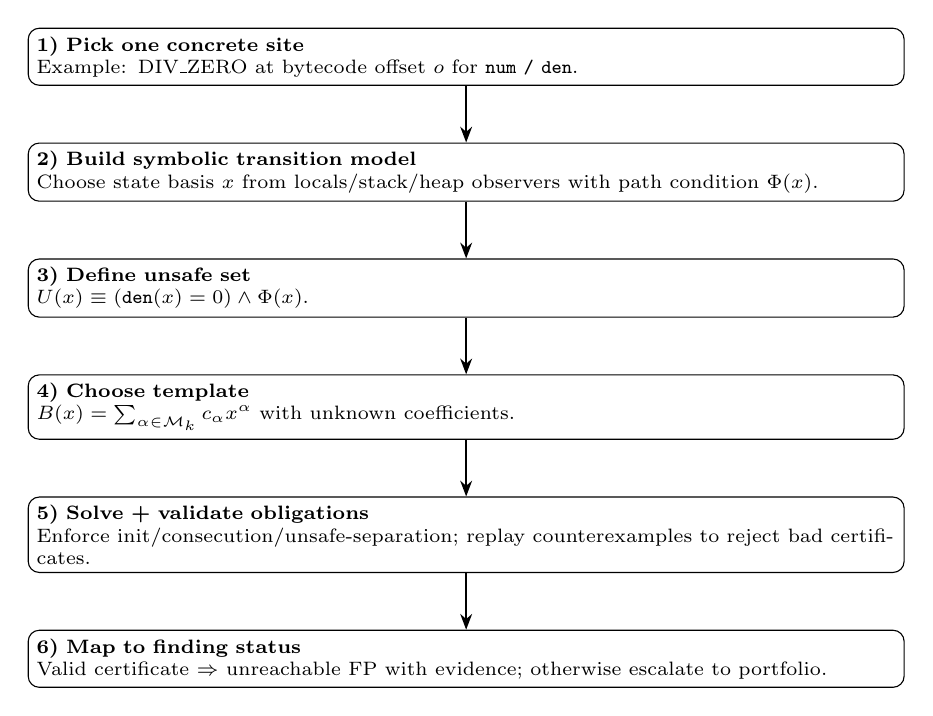
\begin{tikzpicture}[
  node distance=0.72cm,
  box/.style={draw, rounded corners, align=left, font=\scriptsize, inner sep=3pt, text width=0.90\linewidth},
  arr/.style={-{Stealth[length=2mm]}, thick}
]
  \node[box] (a) {\textbf{1) Pick one concrete site}\\
  Example: DIV\_ZERO at bytecode offset $o$ for \texttt{num / den}.};
  \node[box, below=of a] (b) {\textbf{2) Build symbolic transition model}\\
  Choose state basis $x$ from locals/stack/heap observers with path condition $\Phi(x)$.};
  \node[box, below=of b] (c) {\textbf{3) Define unsafe set}\\
  $U(x) \equiv (\texttt{den}(x)=0) \land \Phi(x)$.};
  \node[box, below=of c] (d) {\textbf{4) Choose template}\\
  $B(x)=\sum_{\alpha\in\mathcal{M}_k} c_\alpha x^\alpha$ with unknown coefficients.};
  \node[box, below=of d] (e) {\textbf{5) Solve + validate obligations}\\
  Enforce init/consecution/unsafe-separation; replay counterexamples to reject bad certificates.};
  \node[box, below=of e] (f) {\textbf{6) Map to finding status}\\
  Valid certificate \(\Rightarrow\) unreachable FP with evidence; otherwise escalate to portfolio.};

  \draw[arr] (a) -- (b);
  \draw[arr] (b) -- (c);
  \draw[arr] (c) -- (d);
  \draw[arr] (d) -- (e);
  \draw[arr] (e) -- (f);
\end{tikzpicture}
\end{frame}

\begin{frame}{7. Episode III: Python reality constraints}
\begin{itemize}
  \item Bytecode-level control flow, not source-level wishful semantics
  \item Explicit normal and exceptional transitions (try/except/finally behavior)
  \item Unknown/library behavior modeled with conservative contracts
  \item Executable semantics is the filter that kills elegant but unsound theory
\end{itemize}
\end{frame}

\begin{frame}{8. Short technical example from the blog}
\begin{itemize}
  \item Claim: ``failing assertion escapes uncaught'' is a reachability question
  \item Depends on assert-enable mode, enclosing handlers, caller handlers, finally edges
  \item Naive detector over-reports; theorem-only model under-specifies runtime
  \item Resolution pattern: precise-enough semantics + conservative proof obligations
\end{itemize}
\end{frame}

\begin{frame}{9. The real engine: theorize \(\rightarrow\) code \(\rightarrow\) test \(\rightarrow\) fix code \(\rightarrow\) fix theory}
\begin{enumerate}
  \item AI theorizing proposes abstractions/proof templates quickly
  \item Analyzer implementation exposes semantic and cost pathologies
  \item Synthetic + regression + repo scans provide hard falsification pressure
  \item Code fixes remove operational defects
  \item Theory fixes tighten assumptions/obligations and restart the loop
\end{enumerate}
\end{frame}

\begin{frame}{10. What shipped: static-first, agentic-second}
\begin{itemize}
  \item Static stage performs bulk discovery, disproof/proof, dedup, confidence, SARIF
  \item Agentic stage inspects only unresolved survivors with repository context tools
  \item Design asymmetry: high-assurance methods consume high-volume workload
  \item LLM does not override upstream proof/disproof artifacts
\end{itemize}
\end{frame}

\begin{frame}{11. Transition system used by the analyzer}
\begin{itemize}
  \item State \(\sigma=(pc,\rho,h,\tau,\kappa,e,\Phi)\): control, env, heap, taint, stack, exception mode, path condition
  \item Step relation \(\sigma\xrightarrow{}\sigma'\) split by opcode class and edge type
  \item Control metadata stays concrete; value/flow uncertainty stays symbolic
  \item Unsafe predicate family \(U_t(\sigma)\) indexed by bug type
\end{itemize}
\end{frame}

\begin{frame}{12. What is concretely encoded}
\begin{itemize}
  \item Program counter per frame is concrete integer offset
  \item Locals/stack values are symbolic terms with type tags
  \item Heap observers (length/has-key/type predicates) become solver-visible terms
  \item Exception mode and handler context are first-class transition components
\end{itemize}
\end{frame}

\begin{frame}{13. Kitchensink portfolio}
\begin{itemize}
  \item Principle: orchestrate strong methods; do not worship one paper
  \item Route by bug shape and cost: cheap-strong checks first, expensive methods later
  \item Families: barriers/SOS tiers, induction, CHC/PDR, CEGAR/interpolation, synthesis heuristics
  \item Method disagreement is signal; preserve orthogonal cross-checks
\end{itemize}
\end{frame}

\begin{frame}{13b. Barrier obligations are the unifying interface}
\begin{block}{Every method answers one question about \(B\)}
\(\text{init}: \forall s\in S_0: B(s)\ge\epsilon\quad
\text{consec}: T\land B\ge0\Rightarrow B'\ge0\quad
\text{sep}: \forall s\in U: B(s)\le-\epsilon\)
\end{block}
\begin{itemize}
  \item The barrier certificate defines \textbf{three provable obligations}
  \item Each paper in the portfolio is a specialised solver for one or more of these
  \item Composing them is coherent, not eclectic: every method either \emph{validates} an obligation, \emph{refutes} a candidate, or \emph{narrows the template space}
  \item Failure of any single method is a signal to route to the next, not a project failure
\end{itemize}
\end{frame}

\begin{frame}[shrink=52]{13c. Separation obligation: foundations (papers 1--5)}
\begin{block}{Obligation: \(\forall s\in U: B(s)\le-\epsilon\) and \(B(x)\ge 0\) on reachable region}
\end{block}
\begin{itemize}
  \item \textbf{Stengle 1974} (Positivstellensatz) --- algebraic infeasibility certificate over semialgebraic sets;\\
    \textcolor{blue!75!black}{\textit{BSP: existence guarantee --- if safe/unsafe are truly disjoint, a polynomial fence \(B\) must exist}}\\
    \textcolor{orange!80!black}{\textit{Bent: pure real algebraic geometry with no program semantics; we map program state variables to the polynomial ring and interpret \texttt{assert} guards and error conditions as semialgebraic sets}}
  \item \textbf{Parrilo 2000} (SOS programming) --- polynomial positivity reformulated as SDP via Gram matrix;\\
    \textcolor{blue!75!black}{\textit{BSP: the computational engine --- turns ``fence exists'' into ``we can solve for \(B\)'s coefficients''}}\\
    \textcolor{orange!80!black}{\textit{Bent: Parrilo's domain is continuous nonlinear control (Lyapunov for ODEs); we substitute the ODE state space with RISE's symbolic machine state \(\sigma\), leaving the SDP untouched}}
  \item \textbf{Lasserre 2001} (moment/SOS hierarchy) --- iterative degree lifting to global optimum;\\
    \textcolor{blue!75!black}{\textit{BSP: if degree-\(d\) certificate fails, escalate to degree-\(d{+}2\); hierarchy guarantees convergence}}\\
    \textcolor{orange!80!black}{\textit{Bent: originally a polynomial \emph{optimisation} framework; we repurpose it as a \emph{feasibility-escalation} schedule --- each level is a portfolio tier, not an optimisation step}}
  \item \textbf{Prajna \& Jadbabaie HSCC 2004} (barrier certificates) --- first explicit init/consec/separation triple;\\
    \textcolor{blue!75!black}{\textit{BSP: this \emph{is} the paradigm --- they wrote the three-obligation API we use verbatim over symbolic state}}\\
    \textcolor{orange!80!black}{\textit{Bent: uses Lie-derivative consecution (\(\dot B\ge0\) along ODE flow); we replace this with symbolic one-step \(B(\sigma')\ge0\) under the discrete transition relation \(T\)}}
  \item \textbf{Prajna, Jadbabaie \& Pappas TAC 2007} (stochastic barrier) --- consecution as expectation inequality;\\
    \textcolor{blue!75!black}{\textit{BSP: extends consecution to \(E[B(s')\mid s]\ge0\) for probabilistic transitions and hybrid paths}}\\
    \textcolor{orange!80!black}{\textit{Bent: replaces It\^{o} calculus over SDEs with Python probabilistic branching; expectation computed over path-condition probability mass, not stochastic differentials}}
\end{itemize}
\end{frame}

\begin{frame}[shrink=24]{13d. Separation tractability: relaxation ladder (papers 6--8)}
\begin{block}{Problem: exact SOS/SDP is expensive at high degree or many variables}
\end{block}
\begin{itemize}
  \item \textbf{Ahmadi \& Majumdar SIAM Rev.~2019} (DSOS/SDSOS) --- LP/SOCP relaxations of SOS cone;\\
    \textcolor{blue!75!black}{\textit{BSP: \(B\) still satisfies all three obligations --- the fence is sound, just certified faster via LP instead of SDP}}\\
    \textcolor{orange!80!black}{\textit{Bent: original targets robotics trajectory optimisation (control design); we use DSOS purely as a certificate-existence check, discarding the control objective entirely}}
  \item \textbf{Waki, Kim, Kojima \& Muramatsu 2006} (correlative sparsity) --- decompose SDP along variable correlation graph;\\
    \textcolor{blue!75!black}{\textit{BSP: Python variables rarely all interact; build \(B\) over small local clusters, not the full \(n\)-dimensional State space}}\\
    \textcolor{orange!80!black}{\textit{Bent: original graph built from polynomial support structure; we build it from Python \emph{data-flow} --- two variables co-appear iff they share a branch predicate or arithmetic expression in the RISE IR}}
  \item \textbf{Ames, Coogan, Egerstedt et al.~CDC 2019} (CBF survey) --- continuous consecution as \(\dot B\ge{-}\alpha(B)\);\\
    \textcolor{blue!75!black}{\textit{BSP: discrete analogue is our transition consecution; CBF slope bound motivates contract overapproximation for unknown calls}}\\
    \textcolor{orange!80!black}{\textit{Bent: smooth continuous dynamics with computable Lie derivatives; we discretise the class-\(\mathcal{K}\) slope bound into a per-call contract \(B(\sigma')\ge B(\sigma)-\alpha(B(\sigma))\) for black-box Python functions}}
\end{itemize}
\textbf{Portfolio use:} run DSOS tier first; escalate to full SOS/SDP only on failure.
\end{frame}

\begin{frame}[shrink=38]{13e. Consecution obligation: property-directed reachability (papers 9--12)}
\begin{block}{Obligation: \(\forall s\to s': B(s)\ge0 \Rightarrow B(s')\ge0\)}
\end{block}
\begin{itemize}
  \item \textbf{Sheeran, Singh \& St\aa lm\aa rck FMCAD 2000} (k-induction) --- consecution as bounded SAT base+step;\\
    \textcolor{blue!75!black}{\textit{BSP: checks ``does \(B\) stay \(\ge0\) for \(k\) steps then forever?'' --- unrolls induction instead of finding \(B\) explicitly}}\\
    \textcolor{orange!80!black}{\textit{Bent: propositional SAT over hardware bit-vectors; we run SMT over integer/real program variables and upgrade the logic engine, keeping the base/step structure verbatim}}
  \item \textbf{Bradley VMCAI 2011} (IC3) --- inductive frame predicates block bad cubes forward;\\
    \textcolor{blue!75!black}{\textit{BSP: builds \(B\) implicitly as a clause conjunction; each blocked cube is one constraint maintaining the fence}}\\
    \textcolor{orange!80!black}{\textit{Bent: Boolean SAT over hardware registers; we map ``cube'' to a conjunction of LIA predicates over RISE state and replace SAT generalisation with Z3 model-based quantifier instantiation}}
  \item \textbf{Een, Mishchenko \& Brayton FMCAD 2011} (PDR) --- industrial IC3 with generalized counterexamples;\\
    \textcolor{blue!75!black}{\textit{BSP: same implicit \(B\)-as-clause-set at scale; inductive clause sequence serialises into our SARIF proof artifact}}\\
    \textcolor{orange!80!black}{\textit{Bent: ternary-simulation generalisation is hardware-specific; we replace it with SMT-driven predicate weakening and retain only PDR's proof-artifact extraction, mapping the clause sequence to SARIF}}
  \item \textbf{Gurfinkel, Kahsai, Komuravelli \& Navas CAV 2015} (SeaHorn/CHC) --- software safety as CHC;\\
    \textcolor{blue!75!black}{\textit{BSP: CHC solving \emph{is} the consecution obligation written interprocedurally; tighter summaries = smaller CHC bodies}}\\
    \textcolor{orange!80!black}{\textit{Bent: SeaHorn targets C/LLVM; we re-encode CHC bodies for Python's RISE IR; dynamic dispatch requires per-callsite CHC heads rather than per-function, demanding a custom encoding layer}}
\end{itemize}
\end{frame}

\begin{frame}[shrink=44]{13f. Template refinement: CEGAR and interpolants (papers 13--16)}
\begin{block}{Problem: template \(B\) is wrong; counterexample says where}
\end{block}
\begin{itemize}
  \item \textbf{Clarke, Grumberg, Jha, Lu \& Veith CAV 2000} (CEGAR) --- spurious trace \(\Rightarrow\) refine abstraction;\\
    \textcolor{blue!75!black}{\textit{BSP: failed obligation = gap in the fence; CEGAR patches it by adding monomials to the template basis and re-solving}}\\
    \textcolor{orange!80!black}{\textit{Bent: original ``abstraction'' is a boolean program; ours is the polynomial template degree and monomial basis; ``refinement'' adds monomials from the spurious trace instead of boolean predicates}}
  \item \textbf{Ball, Majumdar, Millstein \& Rajamani PLDI 2001} (SLAM) --- CEGAR for C at Windows-driver scale;\\
    \textcolor{blue!75!black}{\textit{BSP: demonstrates that automated fence-gap patching works in real software without manual monomial selection}}\\
    \textcolor{orange!80!black}{\textit{Bent: SLAM's predicate engine is tightly coupled to C boolean abstraction; we take the \emph{architectural} lesson and substitute a polynomial monomial selector for SLAM's boolean predicate engine}}
  \item \textbf{McMillan CAV 2003} (Craig interpolants) --- tightest new predicate extracted from UNSAT proof;\\
    \textcolor{blue!75!black}{\textit{BSP: interpolant = the minimal new monomial closing the gap; derived directly from the failed obligation's UNSAT core}}\\
    \textcolor{orange!80!black}{\textit{Bent: original extracts propositional/linear interpolants for boolean abstraction; we apply SMT interpolation over non-linear arithmetic and map the formula to new monomial terms in the template}}
  \item \textbf{Henzinger, Jhala, Majumdar \& Suresh POPL 2004} (lazy abstraction) --- refine only the failing subtree;\\
    \textcolor{blue!75!black}{\textit{BSP: don't rebuild the entire \(B\) when one part fails --- surgically patch only the template branch that broke}}\\
    \textcolor{orange!80!black}{\textit{Bent: ``subtree'' in BLAST is a CFG node set in boolean abstraction; in our use it is the monomial support region of \(B\) around the failing check, localising the SDP re-solve to a variable sub-cluster}}
\end{itemize}
\end{frame}

\begin{frame}[shrink=48]{13g. Template synthesis \& witness grounding (papers 17--20)}
\begin{block}{Problem: choose the right \(c_\alpha\) and confirm with a concrete trace}
\end{block}
\begin{itemize}
  \item \textbf{Flanagan \& Leino FME 2001} (Houdini) --- optimistic invariant conjecture, prune by counterexample;\\
    \textcolor{blue!75!black}{\textit{BSP: propose many \(c_\alpha\) configs; drop those that fail obligations; fixpoint = the widest valid \(B\)}}\\
    \textcolor{orange!80!black}{\textit{Bent: Houdini proposes boolean invariant \emph{annotations} for ESC/Java; we generate polynomial \emph{coefficient} candidates; pruning oracle is the three-obligation SMT check, not an annotation checker}}
  \item \textbf{Garg, L\"oding, Madhusudan \& Neider CAV 2014} (ICE) --- invariants from pos/neg/implication examples;\\
    \textcolor{blue!75!black}{\textit{BSP: concrete executions seed \(c_\alpha\) values --- the program's own behaviour shapes the fence coefficients}}\\
    \textcolor{orange!80!black}{\textit{Bent: ICE targets general first-order invariants with unrestricted hypothesis class; we restrict to polynomials of bounded degree and the learner returns \(c_\alpha\) coefficient vectors}}
  \item \textbf{Alur, Bodik, Juniwal et al.~FMCAD 2013} (SyGuS) --- template grammar + SMT oracle loop;\\
    \textcolor{blue!75!black}{\textit{BSP: template family = the grammar; three obligation checks = the oracle; SyGuS formalises our coefficient search}}\\
    \textcolor{orange!80!black}{\textit{Bent: SyGuS is entirely generic (bit manipulation, strings, etc.); we instantiate with a monomial grammar and supply all three BSP obligations as the multi-property SMT oracle}}
  \item \textbf{Godefroid, Klarlund \& Sen PLDI 2005} (DART/concolic) --- concrete+symbolic path exploration;\\
    \textcolor{blue!75!black}{\textit{BSP: walks real executions to confirm \(B\ge0\) on live paths and \(B\le{-}\epsilon\) at real unsafe states}}\\
    \textcolor{orange!80!black}{\textit{Bent: DART's goal is \emph{falsification}; we \emph{invert} it to \emph{confirmation} --- driving concolic runs toward certificate violations to validate \(B\ge0\) on all explored paths, not to report bugs}}
\end{itemize}
\textbf{Key:} papers 17--20 fill the ``who proposes \(c_\alpha\)'' gap that pure SOS leaves open.
\end{frame}

\begin{frame}{14. Solver and feasibility policy}
\begin{itemize}
  \item Candidate survives only if \(\Phi \wedge U_t\) is feasible under current abstraction
  \item UNSAT: elimination artifact (why candidate is unreachable)
  \item SAT: retain candidate, optionally seed witness generation
  \item UNKNOWN/timeout: keep candidate conservatively; route to deeper stage
\end{itemize}
\end{frame}

\begin{frame}{15. CEGAR-style refinement loop}
\begin{itemize}
  \item Start coarse to control compute cost
  \item Spurious counterexample \(\Rightarrow\) refine predicates/contracts/context
  \item Recheck obligations under refined abstraction
  \item Stop on proof, witness, or budget boundary
\end{itemize}
\end{frame}

\begin{frame}{16. Unknown calls: soundness vs precision}
\begin{itemize}
  \item Deterministic assumptions for unknown libraries are unsound
  \item Fully nondeterministic assumptions are too noisy
  \item Practical middle: conservative contracts + widening + concolic checks
  \item Precision improves as contracts mature; soundness envelope remains explicit
\end{itemize}
\end{frame}

\begin{frame}{17. DSE/concolic role in the loop}
\begin{itemize}
  \item Symbolic stage filters and structures candidate space
  \item Concolic stage attempts concrete witnesses for unresolved SAT-like survivors
  \item Presence of witness raises actionability confidence
  \item Absence of witness is not safety proof (bounded exploration)
\end{itemize}
\end{frame}

\begin{frame}{18. Agentic-second triage (residual only)}
\begin{itemize}
  \item Agent inspects source context, guards, callers, tests, imports
  \item Produces TP/FP rationale for uncertain residue
  \item This layer is intentionally downstream of proof-capable filtering
  \item Better static evidence produces better triage behavior
\end{itemize}
\end{frame}

\begin{frame}{19. CI ratchet (``not a firehose'')}
\begin{itemize}
  \item Baseline accepts historical findings once
  \item New unaccepted findings fail CI on protected branches
  \item Resolved findings are pruned automatically
  \item Policy meaning: monotonic ``no net new risk'' gate
\end{itemize}
\end{frame}

\begin{frame}{20. Soundness envelope and known limits}
\begin{itemize}
  \item Python dynamism and reflection limit complete static precision
  \item Resource budgets force incompleteness on hardest programs
  \item Unknown external behavior depends on conservative contracts
  \item Claim is engineering-grade precision with explicit assumptions, not omniscience
\end{itemize}
\end{frame}

\begin{frame}{21. Verification checklist}
\begin{itemize}
  \item What is proved: path infeasibility under encoded semantics + assumptions
  \item What is not proved: full language completeness or unlimited-resource reachability
  \item Why trust pruning: obligation traces + solver outcomes + reproducible artifacts
  \item Why trust escalation: conservative keep-on-UNKNOWN/timeout policy
\end{itemize}
\end{frame}

\begin{frame}[fragile]{22. Practical run modes}
\begin{block}{Single command}
\texttt{a3 scan . --triage}
\end{block}
\begin{block}{Explicit staged mode}
\texttt{a3 scan . --output-sarif results.sarif}\\
\texttt{a3 triage --sarif results.sarif --provider github --agentic}
\end{block}
\begin{itemize}
  \item Staged mode is preferred for CI observability and audit trails
\end{itemize}
\end{frame}

\begin{frame}{23. Close + Q\&A}
\begin{itemize}
  \item Architectural claim: static proof/disproof should absorb most decision volume
  \item Operational claim: triage only uncertain residue, never replace proof artifacts
  \item Process claim: CI ratchet enables sustainable rollout in legacy-heavy repos
  \item Open discussion: stronger contracts, nonlinear proof scalability, calibration drift
\end{itemize}
\end{frame}

\end{document}
